\subsubsection{\stid{4.14} ECP SZ: Fast, Effective, Parallel Error-bounded Exascale Lossy Compression for Scientific Data}

\paragraph{Overview}

Extreme scale simulations and experiments are generating more data than can be stored, communicated and analyzed. Error-bounded lossy compressor is critical because it can get a very high compression ratio while still respecting data fidelity based on user's requirement on compression errors. 
%Current lossless compression methods suffer from low compression ratio and do not adequately address the limitations in storage bandwidth and storage space of projected exascale systems. Existing lossy compressors are not covering the needs of many ECP applications.

The VeloC-SZ project is extending and improving the SZ error-bounded lossy compressor for structured and unstructured scientific datasets. SZ offers an excellent compression ratio as well as very low distortion and compression time. Further work is essential, however, to improve our SZ lossy compressor for ECP scientific datasets, while ensuring that user-set error controls are respected. Specifically, we are: (i) optimizing SZ compression ratios, accuracy and speed based on end-user needs (ii) refactoring SZ in C++ to support a composable compression framework and all data types used in ECP applications, (iii) integrating SZ in ECP client applications, (iv) developing the GPU version of SZ which supports multiple supercomputers with different architectures (such as Aurora, Frontier and Summit), and (v) improving robustness and testability. %Our goal is to produce a high-quality lossy compressor responding to the needs of ECP exascale applications and experiment users. To this end, 
We are working with multiple ECP application teams, including ExaSky cosmology teams (HACC), molecular dynamics simulations groups (EXAALT), x-ray laser imaging experimentalists (ExaFEL), and computational chemists (NWChem-X, GAMESS) to optimize SZ for their applications and to harden SZ.

\paragraph{Key Challenges}

SZ faces several key challenges:
\begin{itemize}
\item \textbf{Parameter tuning}: One challenge in optimizing lossy compression for scientific applications is the large
diversity of scientific data, dimensions, scales, and dynamic data changes in both space and time. Each application requires specific parameters tuning and in some cases, a specific compression pipeline, which is non-trivial to implement.
\item \textbf{Implementation \& optimization over GPU}: A second challenge is the sophisticated design in different stages of the SZ (such as data prediction, Huffman tree construction, Huffman encoding), which makes the development of efficient GPU kernels non-trivial. 
\item \textbf{Diverse integration schemes}: A third challenge is the diversity of the integration schemes for the different ECP client applications: HACC integrates SZ in a proprietary I/O library (GIO), Exafel integrates SZ directly in the LCLS data processing pipeline. GAMESS integrates SZ in the application directly replacing some code sections. NWChem-X integrates SZ for checkpoint/restart. 
\item \textbf{Portable support for GPU}: Optimization of SZ for Aurora and Frontier requires writing portable accelerator codes that are non trivial for complex compression pipeline. 
\item \textbf{Improve development robustness and testability}: The SZ testing infrastructure (unit test, correctness test, performance test, regression test, continuous integration) will need to be adapted and its performance optimized for the new C++ implementation. A template based approach must be used to improve robustness, debugging and testability.
\end{itemize}

\paragraph{Solution Strategy}

As for the first challenge, we keep a close communication with ECP application users to understand their specific demands on the lossy compression. For instance, we have a weekly meeting with ECP application teams to discuss the required error bounds, compression speed and quality and integration. We also exploit an adaptive prediction method to optimize the compression quality for diverse datasets. 
%We are also designing and integrating a control loop capable of adjusting compression parameters from user set constraints, in order to find the betsfit configurations based on user's data fidelity requirement. The automatic part of the tuning will use optimization techniques to explore a large potential configuration space.

As for the second challenge, we keep exploring the new strategies to improve the GPU kernel performance for different stages of SZ. This requires in-depth understanding of SZ compression principles, the pros and cons of each step and thorough knowledge about efficient GPU kernel implementation.  

As for the third challenge, we refactor SZ in C++, starting from the current C version. This refactoring is the perfect occasion to implement a new more modular design of SZ, capable of integrating more stages in the compression pipeline and of selecting compression stages based on specific application data features.

Concerning the fourth challenge, we are in contact with ALCF and OLCF as well as with vendors to access simulators and early systems that will help to optimize the accelerator implementations. The portable GPU implementation of SZ relies on Kokkos.

Concerning the robustness and testability, we are continuously developing and improving it. We will need to adapt it for C++ as part of the SZ refactoring. We will use ECP testing environment when it becomes available. We also often discuss potential solutions with application teams when needed. 

%As for the last challenge, our weekly meetings with the application teams provide us a clear understanding of the integration pathway as well as the expected performance. 

\paragraph{Recent Progress}

We have created an official website (http://szcompressor.org) to organize different versions/products of SZ (such as CPU version, GPU version). The current flagship products include CPU version of SZ (the classic C version), composable version of SZ (a.k.a., SZ3 in C++), CUDA version of SZ, and Kokkos version of SZ. They are all open source libraries under the BSD3 license.

The CPU version of SZ is the classic state-of-the-art version (a.k.a., SZ 2), whose latest version number is 2.1.10. We keep improving SZ 2 to fit user's diverse requirements from different applications. For example, the new features in 2.1.10 include:  the support of user-parameters in python binding particularly for EXAFEL, support for compressing data according to the highest dimension for the specific 3D datasets with high smoothness on the highest dimension; support for fix-value-range; support for printing the statistics related to compression for a better understanding of the compressibility. %SZ 2 has been tested or integrated in many ECP applications, such as HACC, NYX, EXAALT, NWCHEM, and QMCPACK. 

SZ 3 breaks down different stages of SZ to form a loosely-coupled model, such that the users can construct a new compressor by customizing each compression step conveniently. By leveraging SZ 3, the new compression method (published in HPDC2020) leverages a more advanced prediction method by combining the second-order Lorenzo and second-order regression. %Figure \ref{fig:sz-principle} (a) illustrates the design overview of the new compressor based on the SZ model and Figure \ref{fig:sz-principle} (b) demonstrates the significant improvement in compression ratio. 
The compression ratio can be improved by 51\% with the same data distortion level (PSNR) for the ECP QMCPack application dataset.  

%\begin{figure}[htb]
%\centering
%\includegraphics[width=2.8in]{projects/2.3.4-DataViz/2.3.4.14-VeloC-SZ/autotune-arc.eps}
%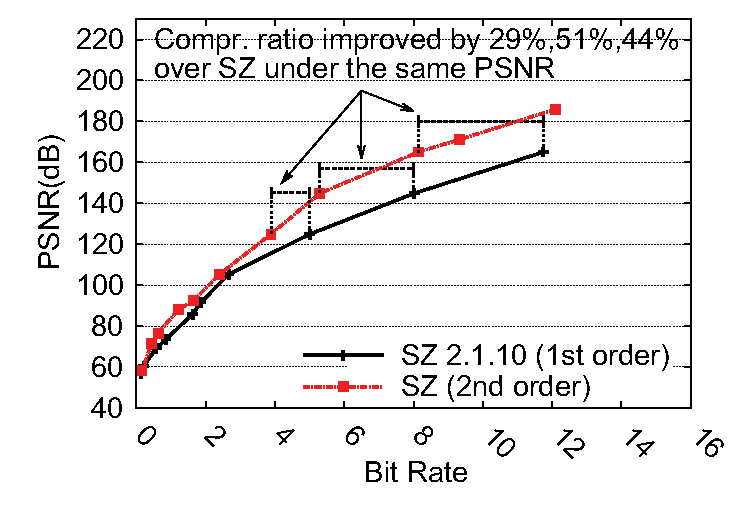
\includegraphics[width=2in]{projects/2.3.4-DataViz/2.3.4.14-VeloC-SZ/qmcpackbig-a.eps}
%\vspace{-2mm}
%	\caption{\label{fig:sz-principle} SZ with 2nd-order predictors and its improvement on rate distortion for QMCPack}
%\end{figure}

We also significantly improved the GPU kernel performance of SZ. We have released the cuda-based SZ (cuSZ) 0.1.1 and tested its performance on V100 GPU (adopted by Summit). The cuSZ is optimized on each compression stage in the SZ framework, including the data prediction, quantization, and Huffman encoding. Specifically, we developed a dual-quantization scheme to entirely remove the data dependency in the prediction step of SZ such that this step can be performed efficiently on GPUs. We developed an efficient customized Huffman coding for the SZ compressor on GPUs. We implemented cuSZ using CUDA and optimized its performance by improving the utilization of GPU memory bandwidth. Figure \ref{fig:cuSZ:arch} presents the design overview, and the technical details can be found in our paper published in PACT2020. Experiments on V100 GPU show that the overall compression performance reaches up to 37GB/s based on both HACC and NYX simulation datasets.

\begin{figure}
  \centering
  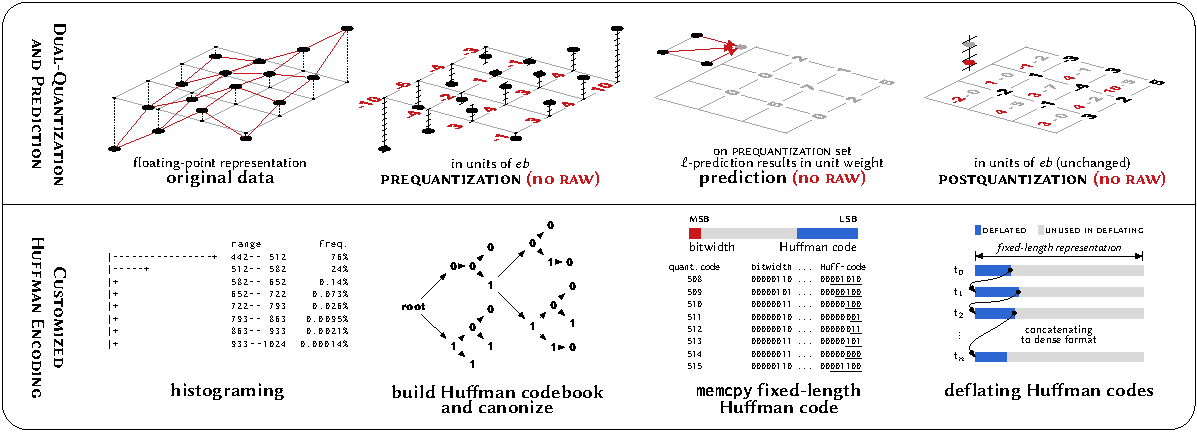
\includegraphics[width=0.8\textwidth]{projects/2.3.4-DataViz/2.3.4.14-VeloC-SZ/200718_workflow.pdf}
  \caption{cuSZ: Design Overview}%
  \label{fig:cuSZ:arch}%
  \vspace{-2mm}
\end{figure}

We also developed the first prototype of kSZ (short for kokkosSZ), and compared its performance to cuSZ (the CUDA version of SZ) on Summit with CUDA GPUs (i.e., NVIDIA Tesla V100) at OCLF. Kokkos provides a good abstraction for both parallel execution of code and data management, which can be used to support portable implementation across different accelerator technologies. The kSZ exhibits performance very similar ($\sim$1\% difference) to cuSZ based in our experiments on Summit.
%Kokkos now can use OpenMP/Pthreads/CUDA (officially released) and OpenMPTarget/oneAPI as backend programming models, so kSZ is able to run on different supercomputers systems each with different GPUs. 

%We also have a good progress on the integration of SZ into EXAALT project. We have developed a multi-level cache system, which exhibits on  

\paragraph{Next Steps} Our next efforts are: (1) Improve compression quality and performance for both cuSZ and kSZ, as well as their stability, (2) keep refactoring SZ in C++ (the first version will be released in Jan, 2021), (3) keep working on the compression quality improvement and integration of SZ in more ECP applications such as EXAALT, and (4) evaluate the portable GPU version of SZ on more ECP platforms.

%\textbf{Support advanced error controls allowing the user to specify relative error bounds and to control the error distribution.} We will write a report describing the integration of additional error controls (relative error bound and control of error distribution) in SZ.
